\documentclass[12pt,a4paper]{article}
\usepackage[utf8]{inputenc}
\usepackage[danish]{babel}
\usepackage[dvipsnames,table]{xcolor}
\usepackage{tikz}
\usetikzlibrary{shapes}
\usetikzlibrary{calc}
\usepackage{anyfontsize}
\usepackage{listings}
\usepackage{float}
\usepackage{url}
\usepackage{graphicx}
\graphicspath{{./img/flowchart/}{./img/test/}{../Flowcharts/}}

\usepackage{changepage}
\usepackage{subcaption}

\usepackage{longtable}
\usepackage{tabularx}
\newcolumntype{b}{X}
\newcolumntype{s}{>{\hsize=.5\hsize}X}

\usepackage{booktabs}

\usepackage{import}
\usepackage{xifthen}
\usepackage{pdfpages}
\usepackage{transparent}

\newcommand{\incfig}[1]{%
    \def\svgwidth{\columnwidth}
    \import{./Flowcharts/}{#1.pdf_tex}
    }

\definecolor{backcolour}{RGB}{245, 245, 245}

\lstdefinestyle{mystyle}{
    backgroundcolor=\color{backcolour},   
    commentstyle=\color{Gray},
    keywordstyle=\color{RoyalBlue},
    numberstyle=\tiny\color{Gray},
    stringstyle=\color{Green},
    basicstyle=\ttfamily\footnotesize,
    breakatwhitespace=false,         
    breaklines=true,                 
    captionpos=b,                    
    keepspaces=true,                 
    numbers=left,                    
    numbersep=5pt,                  
    showspaces=false,                
    showstringspaces=false,
    showtabs=false,                  
    tabsize=2
}

\lstset{style=mystyle}

\newenvironment{changemargin}[2]{%
\begin{list}{}{%
\setlength{\topsep}{0pt}%
\setlength{\leftmargin}{#1}%
\setlength{\rightmargin}{#2}%
\setlength{\listparindent}{\parindent}%
\setlength{\itemindent}{\parindent}%
\setlength{\parsep}{\parskip}%
}%
\item[]}{\end{list}}

\begin{document}

\begin{titlepage}
    
    \pagestyle{empty}

    
\begin{tikzpicture}[remember picture,overlay]

        \fill[YellowOrange] (current page.south west) rectangle (current page.north east);

        \begin{scope}

            \foreach \i in {2.5,...,22}
                {
                    \node[rounded corners,YellowOrange!90,draw,regular polygon,regular polygon sides=6, minimum size=\i cm,ultra thick] at ($(current page.west)+(2.5,-5)$) {} ;

                }

        \end{scope}

        \node[rounded corners,fill=YellowOrange!95,text =YellowOrange!5,regular polygon,regular polygon sides=6, minimum size=2.5 cm,inner sep=0,ultra thick] at ($(current page.west)+(2.5,-5)$) {\LARGE \bfseries \today};

        \foreach \i in {0.5,...,22}
            {
                \node[rounded corners,YellowOrange!90,draw,regular polygon,regular polygon sides=6, minimum size=\i cm,ultra thick] at ($(current page.north west)+(2.5,0)$) {} ;

            }

        \foreach \i in {0.5,...,22}
            {
                \node[rounded corners,YellowOrange!98,draw,regular polygon,regular polygon sides=6, minimum size=\i cm,ultra thick] at ($(current page.north east)+(0,-9.5)$) {} ;
            }

        \foreach \i in {12}
            {
                \node[fill = YellowOrange,rounded corners,draw=YellowOrange,regular polygon,regular polygon sides=6, minimum size=\i cm,ultra thick] at ($(current page.south east)+(-0.2,-0.45)$) {} ;
            }

        \foreach \i in {21,...,6}
            {
            \node[YellowOrange!95,rounded corners,draw,regular polygon,regular polygon sides=6, minimum size=\i cm,ultra thick] at ($(current page.south east)+(-0.2,-0.45)$) {} ;
            }

        \node[left,YellowOrange!5,minimum width=0.625*\paperwidth,minimum height=3cm, rounded corners] at ($(current page.north east)+(0,-9.5)$){{\fontsize{25}{30} \selectfont \bfseries Programmerings Eksamensprojekt}};

        \node[left,YellowOrange!10,minimum width=0.625*\paperwidth,minimum height=2cm, rounded corners] at ($(current page.north east)+(0,-11)$){{\Large \textit{Gold Miner}}};

        \node[left,YellowOrange!5,minimum width=0.625*\paperwidth,minimum height=2cm, rounded corners] at ($(current page.north east)+(0,-13)$){{\Large \textsc{Johan Olesen, 17xad}}};

        \node[left,YellowOrange!5,minimum width=0.625*\paperwidth,minimum height=2cm, rounded corners] at ($(current page.north east)+(0,-15)$){{\Large \textsc{Vejleder: Mark Robert Nygaard Moore}}};

    \end{tikzpicture}

\end{titlepage}

\begin{abstract}
    Dette projekt tager udgangspunkt i problemstilling om at sikre overlevelsen af spil bygget på Adobe Flash Player. Projektet rekreere spillet \emph{Golder Miner} fra start 2000. Målet er at have en fungerende version af \emph{Golder Miner} inklusive hovedfunktionerne af spillet. 

    Projektet ente ud i et program, der ligner det klassiske Gold Miner. Det har alle hovedfunktionerne med om at sænke en spiller arm ned gennem jorden og tage fat i mineraler, hvorefter at trække dem op og få penge af dem tilsvarende værdien af det specifikke mineral.
    
    Programmet er kodet i Processing IDE v. 3.5.4 med sproget Processing, som er baseret på Java. 

\end{abstract}

\newpage

\tableofcontents

\newpage

\section{Problemformulering}
    Eftersom Adobe stopper support til Adobe Flash Player i slutningen af 2020, vil en masse gamle Flash spil stoppe med at virke. Dermed rekreere jeg spillet Gold Miner, så man stadig kan spille det i fremtiden.

    Det er i dag et problem, når firmaer, som Adobe, stopper med at understøtte software som Flash Player og lign. Det gør at ekstremt mange kreative ideer og tanker, bliver tabt til historien, da de stykker kode de bygger på ikke længere kan køres sikkert. Og man som hjemmesidevært ikke vil hoste spillene. Desuden vil hjemmesider som \url{y8.com}, \url{miniclip.com} og \url{kongregate.com} miste en stor del af deres spil katalog, hvoraf langt de fleste af disse vil være gamle klassikere.

\section{Funktionsbeskrivelse}
    Programmet er et spil og dermed bruges der brugerinput. Dette er i form af at brugeren bruger tastaturet, navnlig knapperne, \emph{s} og \emph{w} til at bevæge spilleren, og \emph{r} og \emph{q} for henholdsvis gå tilbage til startposition og genstarte spillet. Brugerens input baseres ud fra hans/hendes observation på skærmen. Spil vinduet er $600 \times 600$ px. Dette betyder at man kan spille spillet på siden, mens man laver noget andet, der ikke kræver ens fulde opmærksomhed. Desuden er de grafiske elementer scaleret til at passe i et lille skærmvindue.

    Programmet bruges som et middel for tidsfordriv og afslapning. Ligesom mange andre spil i samme stil, kræver spillet ikke den store koncentration. Der er ikke mulighed for multiplayer, hverken lokalt eller online.

\section{Dokumentation}
    \subsection{Spilletshistorie}
        Princippet i spillet bygger på at brugeren er en guld graver. Brugeren har en kran til at hive mineraler op fra jorden. Brugeren vil gerne tjene penge, og derved vil brugeren helst grave guld op, da man får flere penge af at grave guld op end sten. Da guld er et sjældnere materiale end sten, befinder guldet som for det første i mindre stykker, og for det andet dybere nede. Det betyder at man ofte bliver nødt til at fjerne nogle sten for overhovedet at kunne for fat i alle guldstykkerne.

    \subsection{Detaljeret beskrivelse af Mineral klassen og inheritance konceptet og brugen}
        Mineral klassen skal bevirke som en skabelon til at lave forskellige typer af mineraler udfra. Den skal laves således at man bare kan ændre nogle få variabler i constructoren og derved vil man have et nyt mineral.

        Klassen består således af en constructor og metoder til at vise objektet, gemme det specifikke objekts oplysninger i et array, hvis Player kolliderer med det, til brug som argument for Player metoden '\textbf{grap()}', og til at ændre en variabel for om mineralet er hejset op.

        \begin{figure}[H]
            \centering
            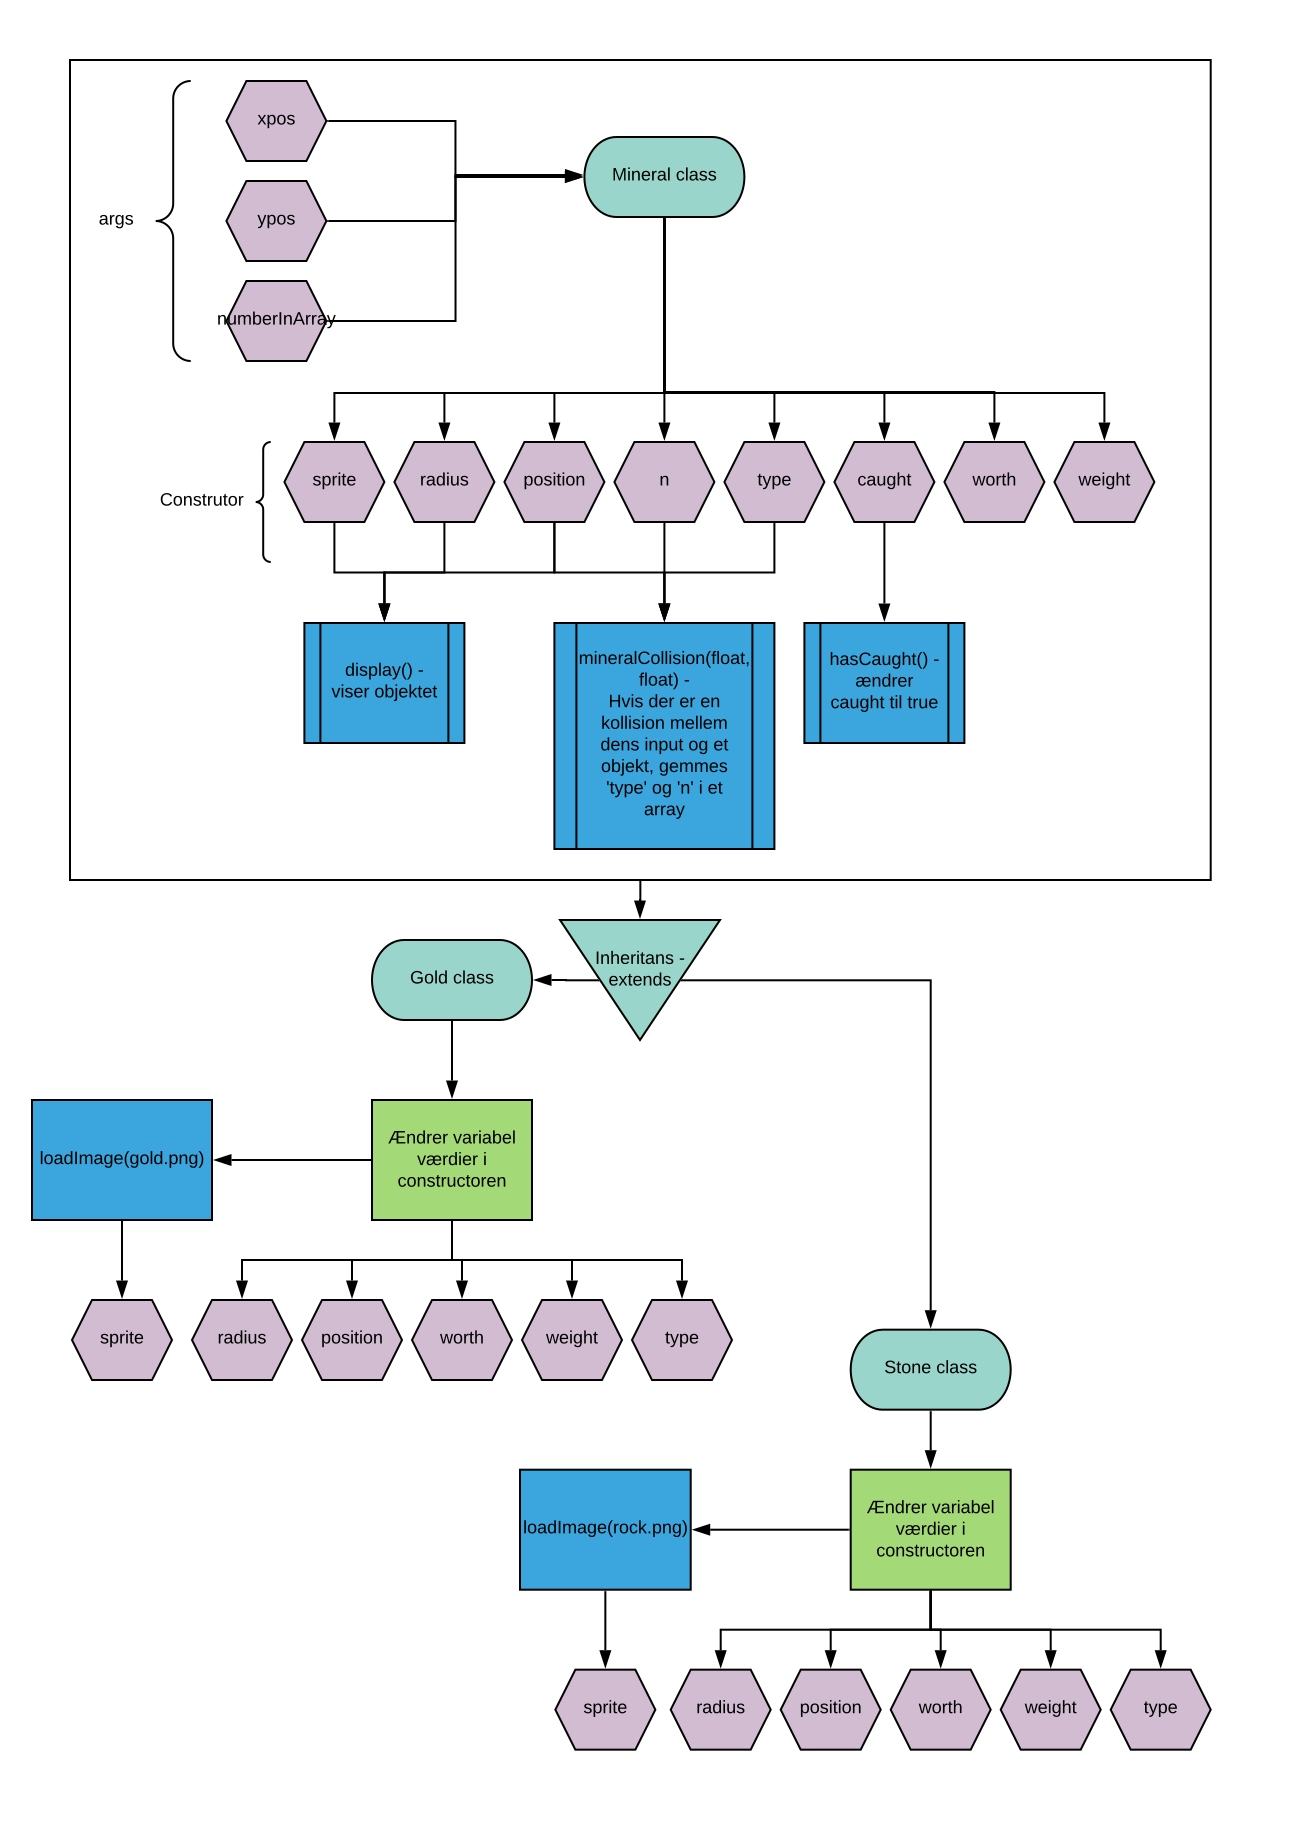
\includegraphics[width=1 \textwidth]{Flowchart - Mineral}
            \caption{Flowchart over Mineral klassen og dens underklasser}
            \label{}
        \end{figure}

        Klassen bruges som sagt som skabelon for de forskellige mineral typer; Stone og Gold. Det gøres ved brug af OOP konceptet omkring nedarvning; \emph{inheritance}. I generel Java kode skrives;
        
        \begin{lstlisting}[language=Java]
class ClassName extends OtherClass {
    ClassName(type args) {
        super(args);
    }
}
\end{lstlisting}
        
        Efter Mineral klassen er skrevet kan man således i en ny klasse bruge inheritance til at nedarve Mineral til den nye klasse. Dette er gjort ved Stone og Gold. 
        \begin{lstlisting}[language=Java, caption=Stone klassen]
class Stone extends Mineral {

    //Load sprite image file.
    PImage r_sprite = loadImage("../sprites/rock.png");
                
    //Constructor changes a few variables.
    Stone(int xpos, int ypos, int numberInArray) {
        super(xpos, ypos, numberInArray);
        ...
    }
}
\end{lstlisting}

        \begin{lstlisting}[language=Java, caption=Gold klassen]
class Gold extends Mineral {
  
    //Load sprite image file.
    PImage g_sprite = loadImage("../sprites/gold.png");
  
    //Constructor changes a few variables.
    Gold(int xpos, int ypos, int numberInArray) {
        super(xpos, ypos, numberInArray);
        ...
    }
}
\end{lstlisting}

    Hvis man så kigger på metoderne i Mineral klassen, ser man at der er tre; 
    \begin{itemize}
        \item display;
\begin{lstlisting}[language=Java]
    void display() {
    imageMode(CENTER);
    image(sprite, x, y, radius, radius);
}
\end{lstlisting}
        display bruges som navnet antyder, til at vise objektet på skærmen. Dette gøres ved brug af Processings funktion, \emph{image()}, der tager en billedefil, et koordinatsæt og en størrelse, som argument. Koordinatsættet er placering på objektet og størrelsen sættes som radius på objektet.

        Man kan se at \emph{display} ikke returner noget, da det har datatypen void, hvilket betyder "manglen på noget", og den tager ikke mod nogen argumenter.
        
        \item mineralCollision;
\begin{lstlisting}[language=Java]
int[] mineralCollision(float a, float b) {
    int[] mineralCollision = new int[2];
    if (dist(a, b, x, y) < radius) {
        mineralCollision[0] = n;
        mineralCollision[1] = type;
    }
    return mineralCollision;
}
\end{lstlisting}

        mineralCollision bruges til at gemme de nødvendige oplysninger om et specifikt objekt til brug i andre funktioner i programmet. Dermed er den sat op til at have en datatype som integer (int). Men for ikke at skulle lave flere funktioner der returnere en integer, har jeg valgt at mineralCollision skal returnere et array af integers. 

        \item hasCaught;
\begin{lstlisting}[language=Java]
boolean hasCaught() {
    return caught = true;
}
\end{lstlisting}

    hasCaught ændrer en variabel for et specifikt Mineral objekt. Variablen der skal ændres er af datatypen boolean, derved skal metoden også returnere en boolean.
    \end{itemize}

    \subsection{Funktion og metode oversigt for GoldMiner}
    \begin{tabularx}{\textwidth} {
        >{\raggedright\arraybackslash}s 
        >{\raggedright\arraybackslash}b 
        >{\raggedright\arraybackslash}s
        >{\raggedright\arraybackslash}s
        >{\raggedright\arraybackslash}b}
        
            \toprule
            \textbf{class} & \textbf{name} & \textbf{type} & \textbf{args} & \textbf{usecase}\\
            \midrule
            Main & settings & void & & Bruges til at sætte indstillingerne for programmet. Heri vinduestørrelse med \emph{size()}. Køres en enkelt gang. \\
            \midrule
            Main & setup & void & & Bygger videre på \emph{settings()} ved at sætte frameraten, loade baggrundsbille, sætte setupphase loopet og tilføje alle Mineral objekterne til ArrayList. Køres en enkelt gang. \\
            \midrule
            Main & draw & void & & Funktion der styrer hovedprogram loopet. \emph{draw} køres hvert frame. \\
            \midrule
            Main & regen & void & & Erstatter Mineral objekter i ArrayList med nye. \\
            \midrule
            Main & overlap & boolean & float, float, float, float, float, float & Tjekker om der er overlap mellem input punkterne. Returner sand hvis og false hvis ikke. \\
    \end{tabularx}
    \begin{tabularx}{\textwidth} {
        >{\raggedright\arraybackslash}s 
        >{\raggedright\arraybackslash}b 
        >{\raggedright\arraybackslash}s
        >{\raggedright\arraybackslash}s
        >{\raggedright\arraybackslash}b}
            \midrule
            Main & keyPressed & void & & Sender tastatur input om en knap er trykket ned til \emph{Player.setMove}. \\
            \midrule
            Main & keyReleased & void & & Sender tastatur input om en knap er sluppet til \emph{Player.setMove}. \\
            \midrule
            Mineral & display & void & & Metoden rendere objektet ved \emph{image()} \\
            \midrule
            Mineral & mineralCollision & int array & float, float & Metoden laver et array på 2. Hvis distancen mellem input argumenterne og Mineral objektets \textit{x} og \textit{y} variabel (koordinater), så sættes $[0] = n$ og $[1] = type$, hvilket betyder at oplysningerne for hvilket Mineral objekt, der er kollideret med input argumenterne, returneres. \\
            \midrule
            Mineral & hasCaught & boolean & & Metoden ændrer variablen, \textit{caught} til \emph{true}, og dermed bliver objektet tagget til at fjernes. \\
    \end{tabularx}
    \begin{tabularx}{\textwidth} {
        >{\raggedright\arraybackslash}s 
        >{\raggedright\arraybackslash}b 
        >{\raggedright\arraybackslash}s
        >{\raggedright\arraybackslash}s
        >{\raggedright\arraybackslash}b}
            \midrule
            Player & display & void & & Del 1 af rendering af objekt. Metoden bruges til at vise objektet ved \emph{circle()}. \\
            \midrule
            Player & update & void & & Del 2 af rendering af objekt. Metoden bruges til at opdatere variablerne som bruges i \emph{display()}. \\
            \midrule
            Player & grap & void & int, int & Metode til at køre metoder og funktioner, når en kollision mellem Player objekt og et Mineral objekt finder sted. Metoderne der køres; \emph{Score.calcMoney}, \emph{Mineral.hasCaught()} og \emph{pReset()}. Samt manipulere med Player objekt, for at trække tilbage automatisk og genstarte \emph{update()}.\\
            \midrule
            Player & setMove & boolean & char, boolean & Et "switch-case" scenarie. Metode til at oversætte tastatur inputs til boolean variabler. \\
    \end{tabularx}
    \begin{tabularx}{\textwidth} {
        >{\raggedright\arraybackslash}s 
        >{\raggedright\arraybackslash}b 
        >{\raggedright\arraybackslash}s
        >{\raggedright\arraybackslash}s
        >{\raggedright\arraybackslash}b}
            \midrule
            Player & movement & void & & Metode til at oversætte boolean variabler fra \emph{setMove()} til objekt variabler og køre \emph{pReset()}. \\
            \midrule
            Player & pReset & void & & Metode til at sætte Player objektet til start værdier. \\
            \midrule
            Score & display & void & & Metoden rendere objektet ved \emph{text()}. \\
            \midrule
            Score & calcMoney & int & int, int & Metode til at beregne hvor meget der skal tilføjes til \emph{money} baseret på et specifikt Mineral objekt. Returnerer \emph{moneyAdd}. \\
            \bottomrule
    \end{tabularx}
   

\newpage

\section{Test af spillet}
    Til at test programmet compiler jeg det og prøver at gennemføre spillet.
    \begin{figure}[H]
        \begin{subfigure}{.5\textwidth}
            \centering
            \includegraphics[width=.98\linewidth]{1.png}
            \caption{Opstart af spillet, med generede mineraler. Player armen svinger frem og tilbage}
        \end{subfigure}
        \begin{subfigure}{.5\textwidth}
            \centering
            \includegraphics[width=.98\linewidth]{2.png}
            \caption{Brugeren trykker \emph{s} og armen rækkes ud}
        \end{subfigure}
        \begin{subfigure}{.5\textwidth}
            \centering
            \includegraphics[width=.98\linewidth]{3.png}
            \caption{Armen har ramt et mineral og trækkes tilbage.}
        \end{subfigure}
        \begin{subfigure}{.5\textwidth}
            \centering
            \includegraphics[width=.98\linewidth]{4.png}
            \caption{Penge bliver tilføjet og armen begynder at svinge igen.}
        \end{subfigure}
        \caption{Gameplay af GoldMiner}
    \end{figure}
    \begin{figure}[H]
        \begin{subfigure}{.5\textwidth}
            \centering
            \includegraphics[width=.98\linewidth]{5.png}
            \caption{Når man har samlet alle mineralerne vises slutskærmen med ens score.}
        \end{subfigure}
        \begin{subfigure}{.5\textwidth}
            \centering
            \includegraphics[width=.98\linewidth]{6.png}
            \caption{Brugeren har trykket \emph{q} og et nyt level starter.}
        \end{subfigure}
        \caption{Slutskærm og ny bane.}
    \end{figure}


    \subsection*{Forbedring / viderebygningsmuligheder}
        \begin{itemize}
            \item \textbf{Opgraderinger}; ind i mellem levels kunne man lave et opgraderingssystem, så man kunne få mulighed for at gøre sin opsamler større så det er lettere at ramme.
            \item \textbf{Flere typer af mineraler}; man kunne introducere flere slags mineraler.
            \item \textbf{Bedre mineral generation}; optimering af valg af placering til mineralerne.
            \item \textbf{Start menu}; en start menu med Spil, How to play og highscores kunne introduceres for at gøre det mere brugervenligt.
            \item \textbf{Sprite til Player}; istedet for en sort streg og lysegrå kugle kunne man give Player en ordentlig sprite ligesom mineralerne.
            \item \textbf{Highscore system}; man kunne implementere et highscore system, der kan gemme ens score og kan man se den i en highscore-menu. 
        \end{itemize}

\section{Konklusion}
    For at konkludere på projektet er der blevet lavet et program, som efter tidsrammen ligner det originale Gold Miner forholdsvist godt. Programmet har stadigvæk en del mangler og kunne bruge en del optimering. 
    
    Spillet har haft indflydelse fra matematik om hvordan punkter beregnes ud fra andre punkter ved hjælp af de trigonometriske funktioner. 

\newpage

\section{Bilag - Flowcharts og source kode}
    \begin{figure}[H]
        \centering
        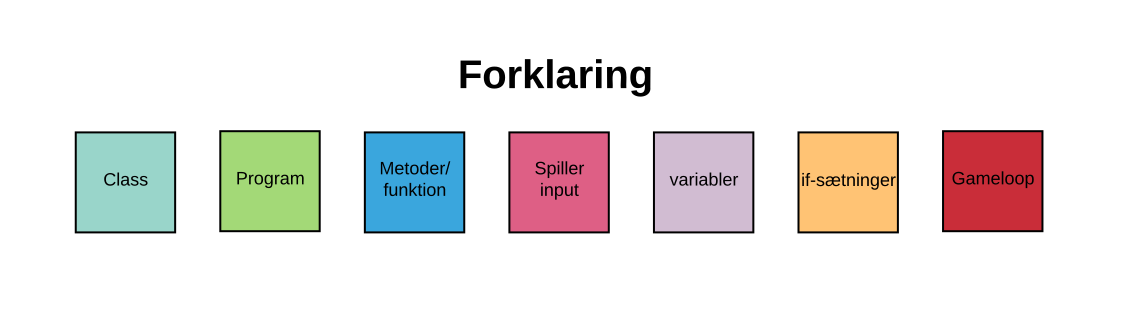
\includegraphics[width=\textwidth]{Flowchart - Forklaring}
    \end{figure}

    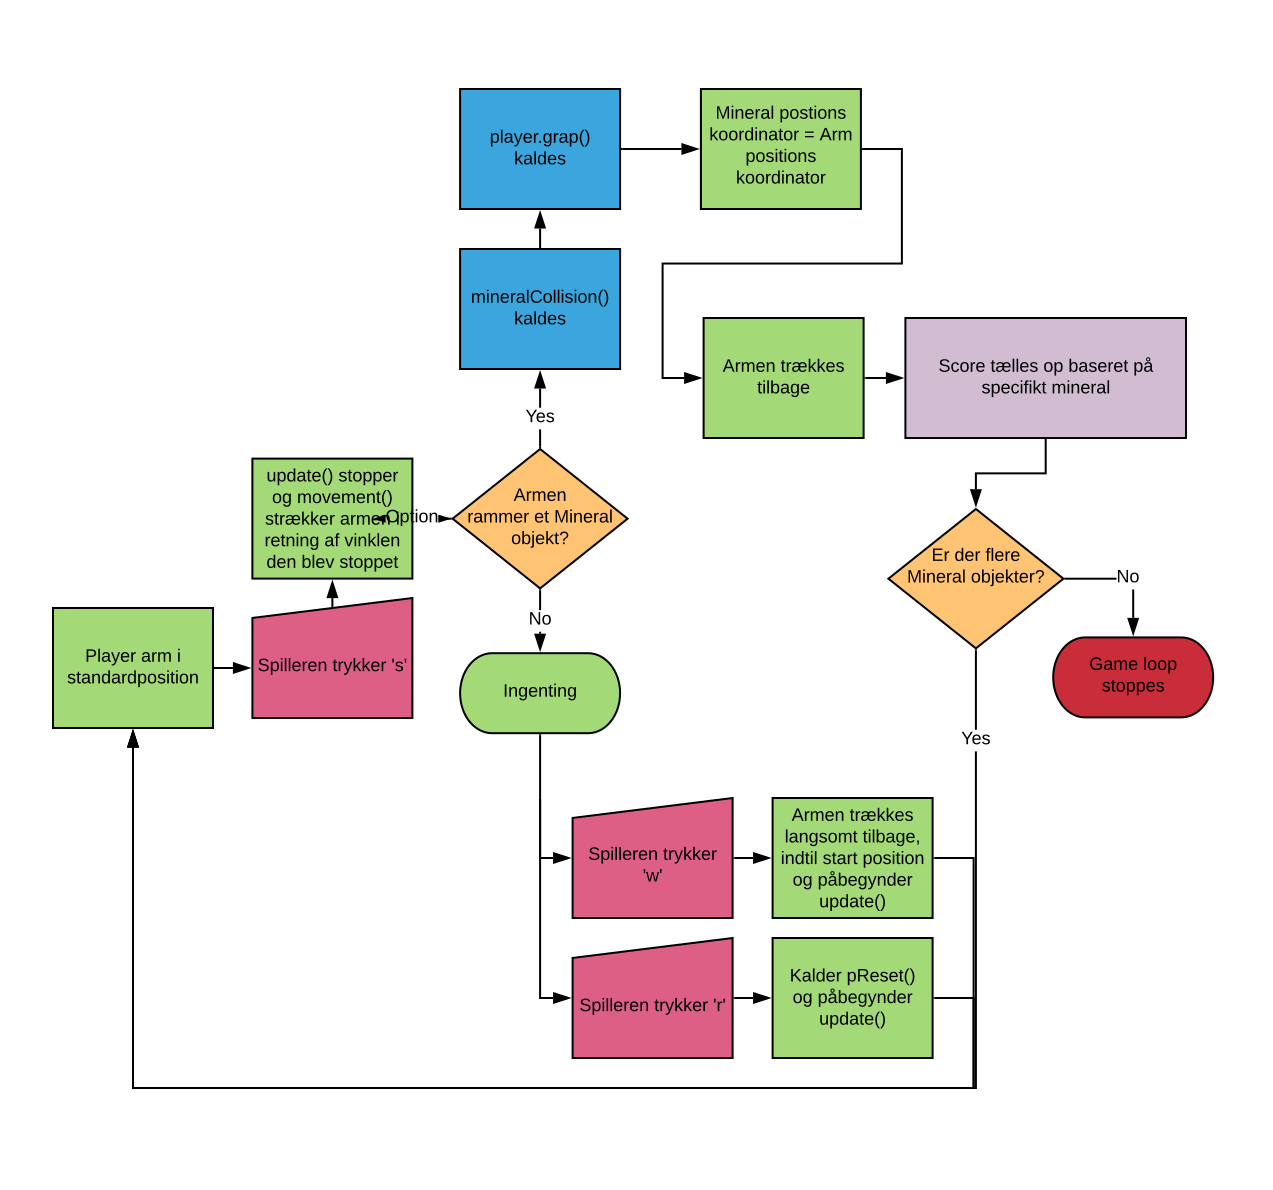
\includepdf{Flowchart - funktionel beskrivelse af bruger scenarie.pdf}
    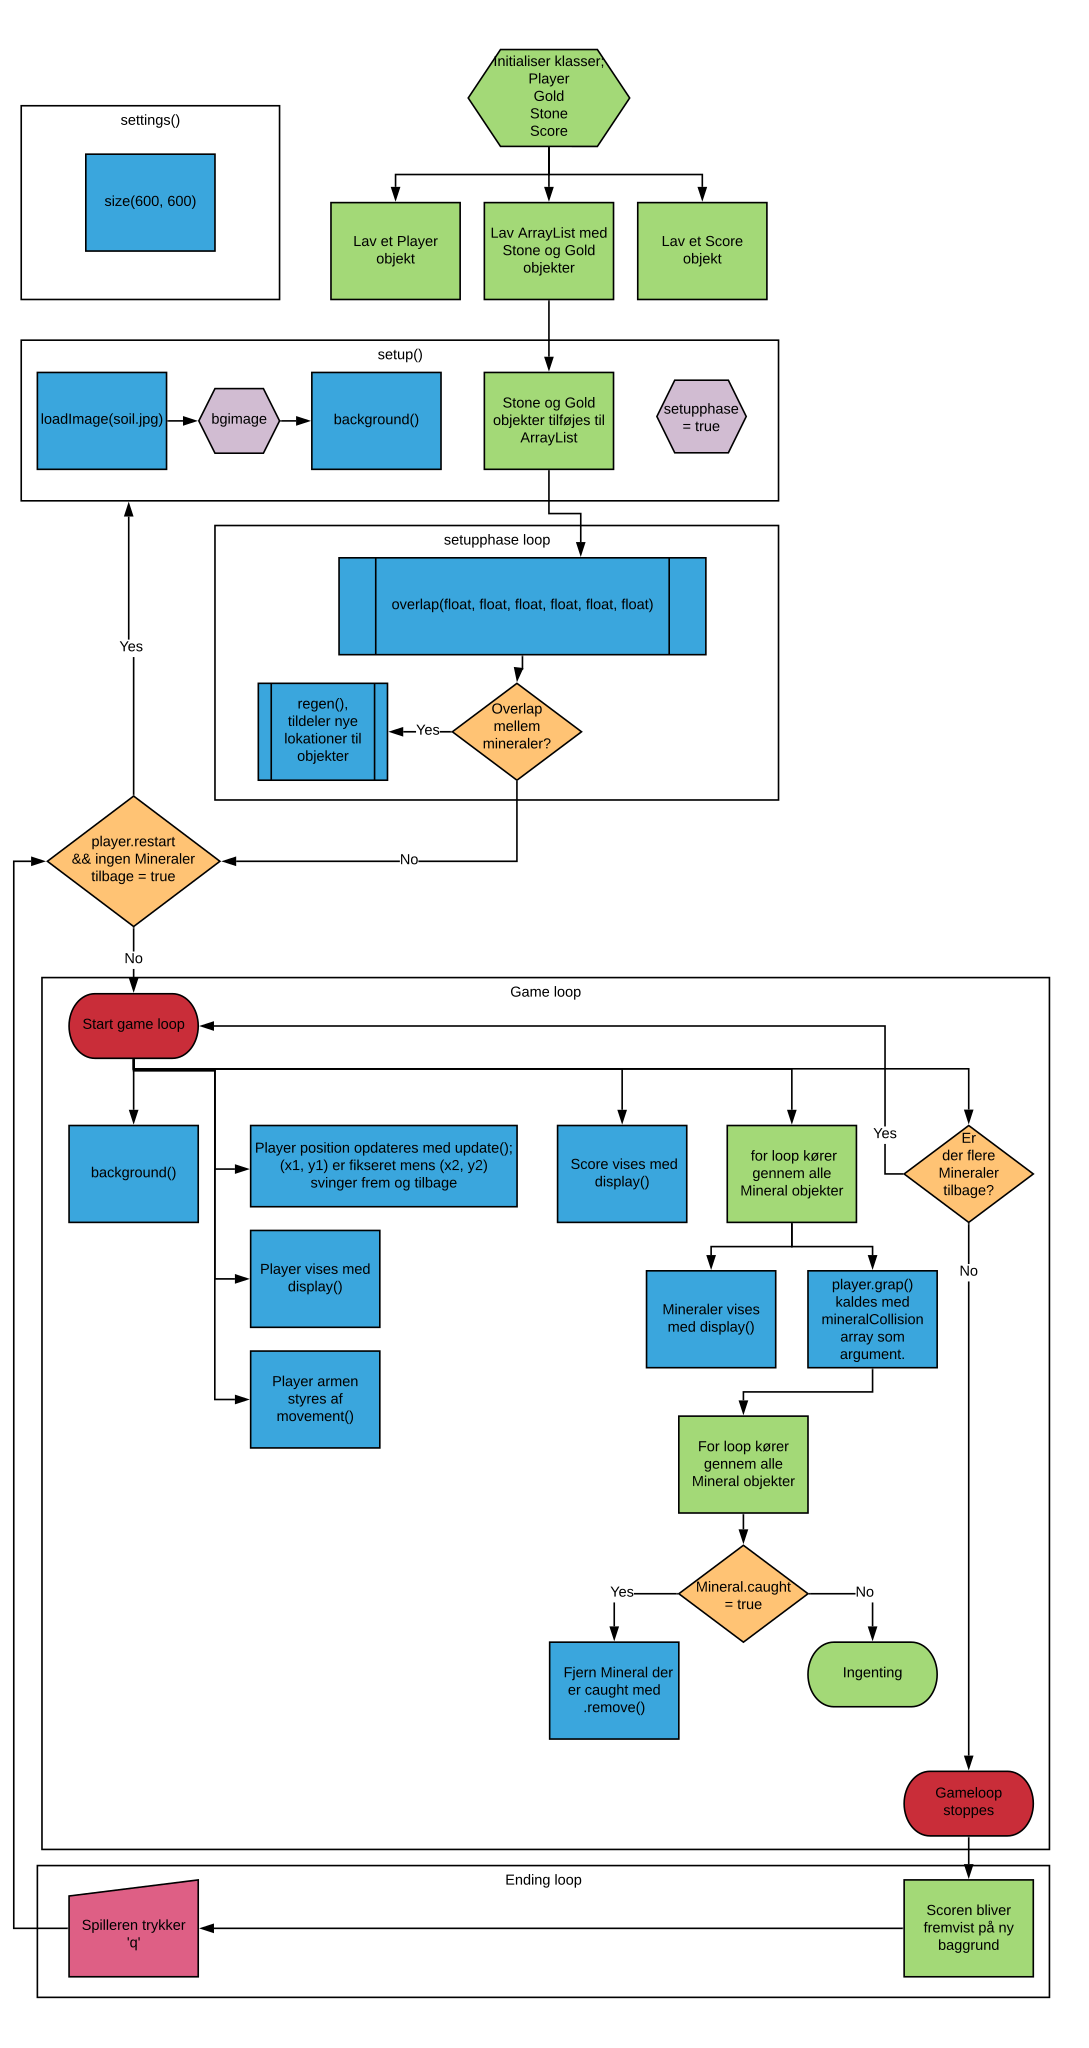
\includepdf{Flowchart - Main.pdf}
    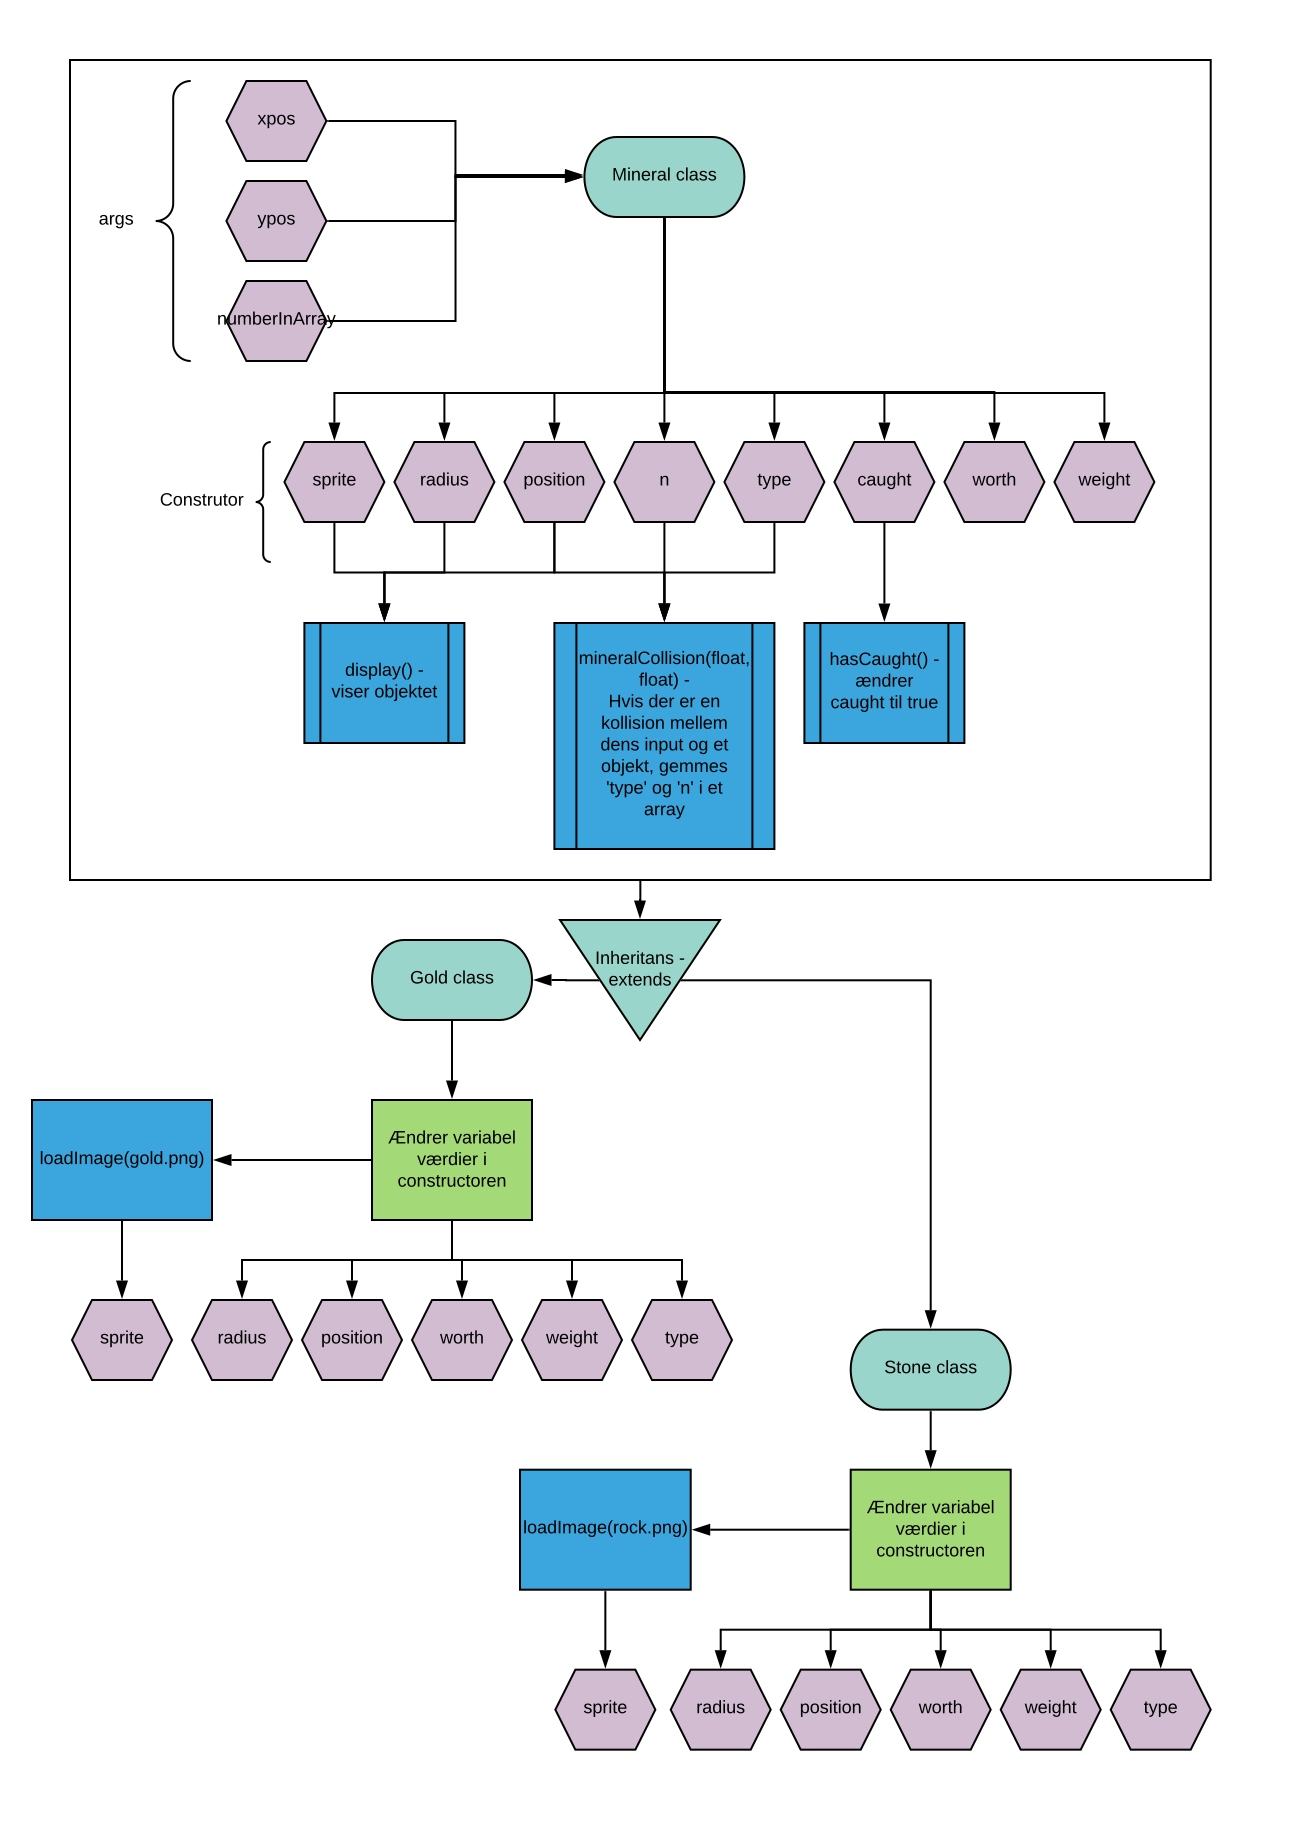
\includepdf{Flowchart - Mineral.pdf}
    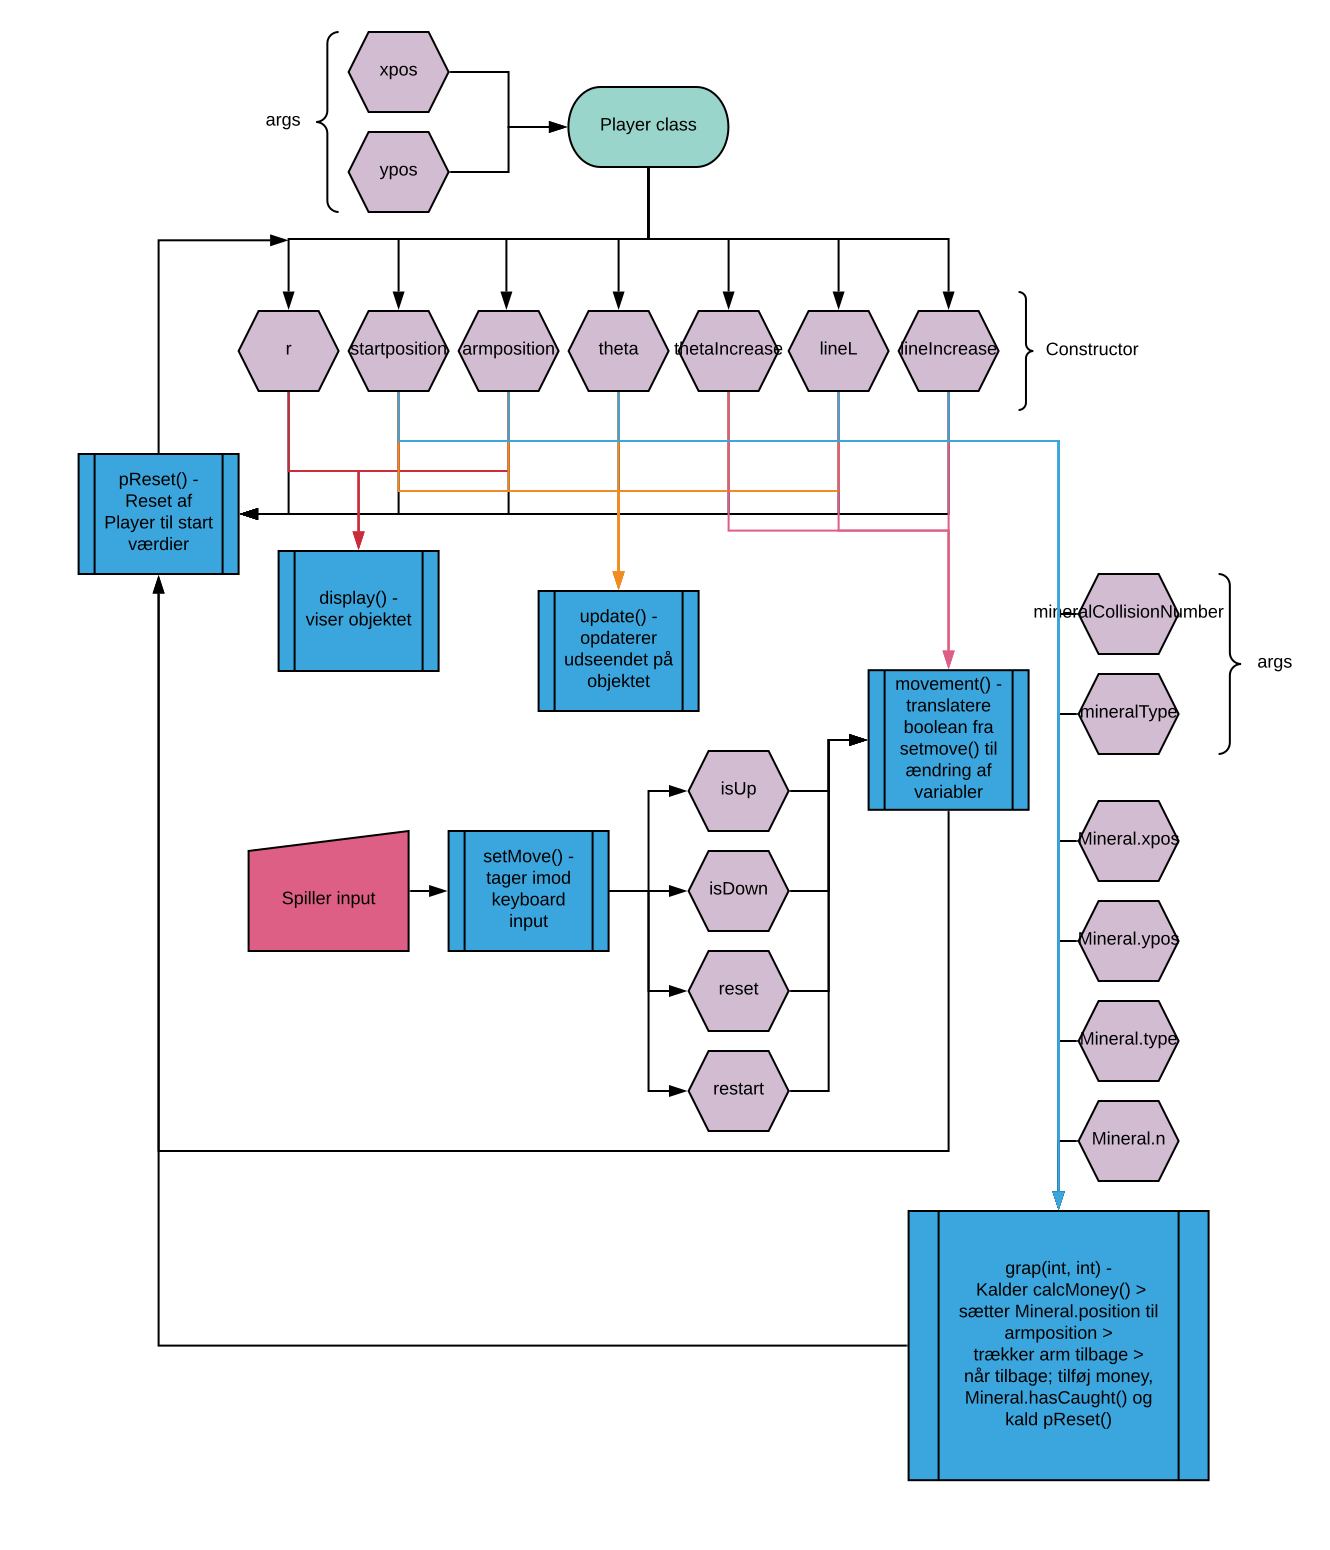
\includepdf{Flowchart - Player.pdf}
    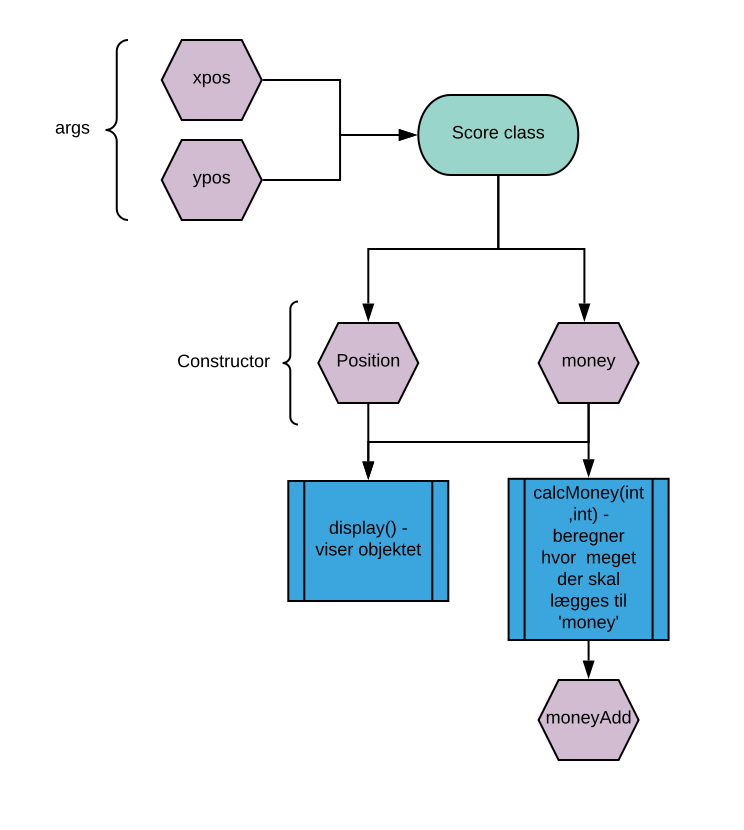
\includepdf{Flowchart - Score.pdf}

    \includepdf[pages=-]{../Source/src_code.pdf}

\end{document}